\documentclass[sn-apa]{sn-jnl}% APA Reference Style 
% \documentclass[sn-apa,iicol]{sn-jnl}% APA Reference Sytle with Double Column

%%%% Standard Packages
%%<additional latex packages if required can be included here>

\usepackage{graphicx}%
\usepackage{multirow}%
\usepackage{amsmath,amssymb,amsfonts}%%%
\usepackage{amsthm}%
\usepackage{mathrsfs}%
\usepackage[title]{appendix}%
\usepackage{xcolor}% shi
\usepackage{textcomp}%
\usepackage{manyfoot}%
\usepackage{booktabs}%
\usepackage{algorithm}%
\usepackage{algorithmicx}%
\usepackage{algpseudocode}%
\usepackage{listings}
\usepackage{rotating}
\usepackage{adjustbox}
\usepackage{booktabs}
\usepackage{longtable}
\usepackage{ltablex}
\usepackage{tabu}
\usepackage{verbatim}
\usepackage{multirow}
\usepackage{hyperref} % For clickable links in the table of contents
\usepackage{tocloft}


%%%% uespackages needed for APA7 style
\usepackage[utf8]{inputenc}
\usepackage[style=apa, backend=biber]{biblatex}
\addbibresource{sn-bibliography.bib}


%% as per the requirement new theorem styles can be included as shown below
\theoremstyle{thmstyleone}%
\newtheorem{theorem}{Theorem}%  meant for continuous numbers
%%\newtheorem{theorem}{Theorem}[section]% meant for sectionwise numbers
%% optional argument [theorem] produces theorem numbering sequence instead of independent numbers for Proposition
\newtheorem{proposition}[theorem]{Proposition}% 
%%\newtheorem{proposition}{Proposition}% to get separate numbers for theorem and proposition etc.

\theoremstyle{thmstyletwo}%
\newtheorem{example}{Example}%
\newtheorem{remark}{Remark}%

\theoremstyle{thmstylethree}%
\newtheorem{definition}{Definition}%

\raggedbottom

%%\unnumbered% uncomment this for unnumbered level heads
\renewcommand{\cftfigpresnum}{Figure\ }
\renewcommand{\cftfigaftersnum}{:}
\setlength{\cftfigindent}{0pt}
\setlength{\cftfignumwidth}{4.5em}

\begin{document}

\title[Reliability SPE ]{Supplementary Material for ``A Multiverse Assessment of the Reliability of the Perceptual Matching Task as a Measurement of the Self-Prioritization Effect"}


\author[1,2]{\fnm{Zheng} \sur{Liu}}
\equalcont{These authors contributed equally to this work.}

\author[1]{\fnm{Mengzhen} \sur{Hu}}
\equalcont{These authors contributed equally to this work.}

\author[1]{\fnm{Yuanrui} \sur{Zheng}}

\author[3]{\fnm{Jie} \sur{Sui}}

\author*[1]{\fnm{Hu} \sur{Chuan-Peng}}\email{hu.chuan-peng@nnu.edu.cn; hcp4715@hotmail.com}

\affil*[1]{\orgdiv{School of Psychology}, \orgname{Nanjing Normal University}, \orgaddress{\city{Nanjing}, \country{China}}}

\affil*[2]{\orgdiv{ School of Humanities and Social Sciences}, \orgname{The Chinese University of Hong Kong-Shenzhen}, \orgaddress{\city{Shenzhen}, \country{China}}}

\affil*[3]{\orgdiv{School of Psychology}, \orgname{University of Aberdeen}, \orgaddress{\city{Old Aberdeen}, \country{Scotland}}}


%%==================================%%
%% sample for unstructured abstract %%
%%==================================%%

\maketitle

\newpage
\tableofcontents
\thispagestyle{empty}
\clearpage

\newpage
\setcounter{page}{1}
\listoffigures
\thispagestyle{empty}
\clearpage

\section{Supplementary Methods}\label{Methods}

\subsection{Methodological details of dataset from \textcite{hu2023data}}\label{ExperimentalDesign}

In this current study, we utilized a dataset that was previously collected by our research team in 2016 \parencite{hu2023data}. The original study aimed to compare SPE between two groups: individuals with sub-clinical depression and those without depression. The dataset comprised data from six time points, each one week apart, collected from a sample of 36 participants recruited from the Tsinghua University community. At each time point, participants completed three distinct tasks: Experiment A (a modified SPMT with large deviation), Experiment B (another modified SPMT with small deviation), and a questionnaire. The original research faced challenges in recruiting sub-clinical depressed participants, leading to an over representation of individuals in the healthy control group, however, making it suitable for the current study. Thus, in our current analysis, we focused on the subset of data related to the neutral condition in Experiment B from these 36 participants. In the following sections we provided a detailed overview of the original experimental design. 

\subsubsection{Ethics Information}\label{subsec:ethics}

The experiment was approved by the IRB at the Department of Psychology, Tsinghua University, and all participants provided informed consent.

\subsubsection{Participants}\label{subsec:participants}

36 participants were recruited from Tsinghua University and nearby community, all of whom were right-handed and had normal or corrected-to-normal vision. Participants were pre-tested for their depressive level by Beck Depression Inventory-II (BDI-II) \parencite{wang2011reliability}. Data from three participants were excluded due to invalid trials or program malfunctions. The exclusion left 33 valid participants ($\text{Mean}_{\text{age}}$ = 21.06, $\text{SD}_{\text{age}}$ = 3.24), with 21 females and 12 males. It's worth noting that within this sample of 33 participants, only six individuals had a BDI-II score exceeding 20.

\subsubsection{Experimental Design}\label{subsec:experimentaldesign}

Experiment 2 was a 2 (Matching: Matching vs. Non-matching) × 3 (Idnetity: Self, Friend, Stranger) × 4 (Emotion: Control, Neutral, Happy, Sad) × 6 (Sessions: 1-6) experiment. 

\renewcommand{\thefigure}{S\arabic{figure}} % Redefine figure label format

\begin{figure}[!ht]
	\centering
	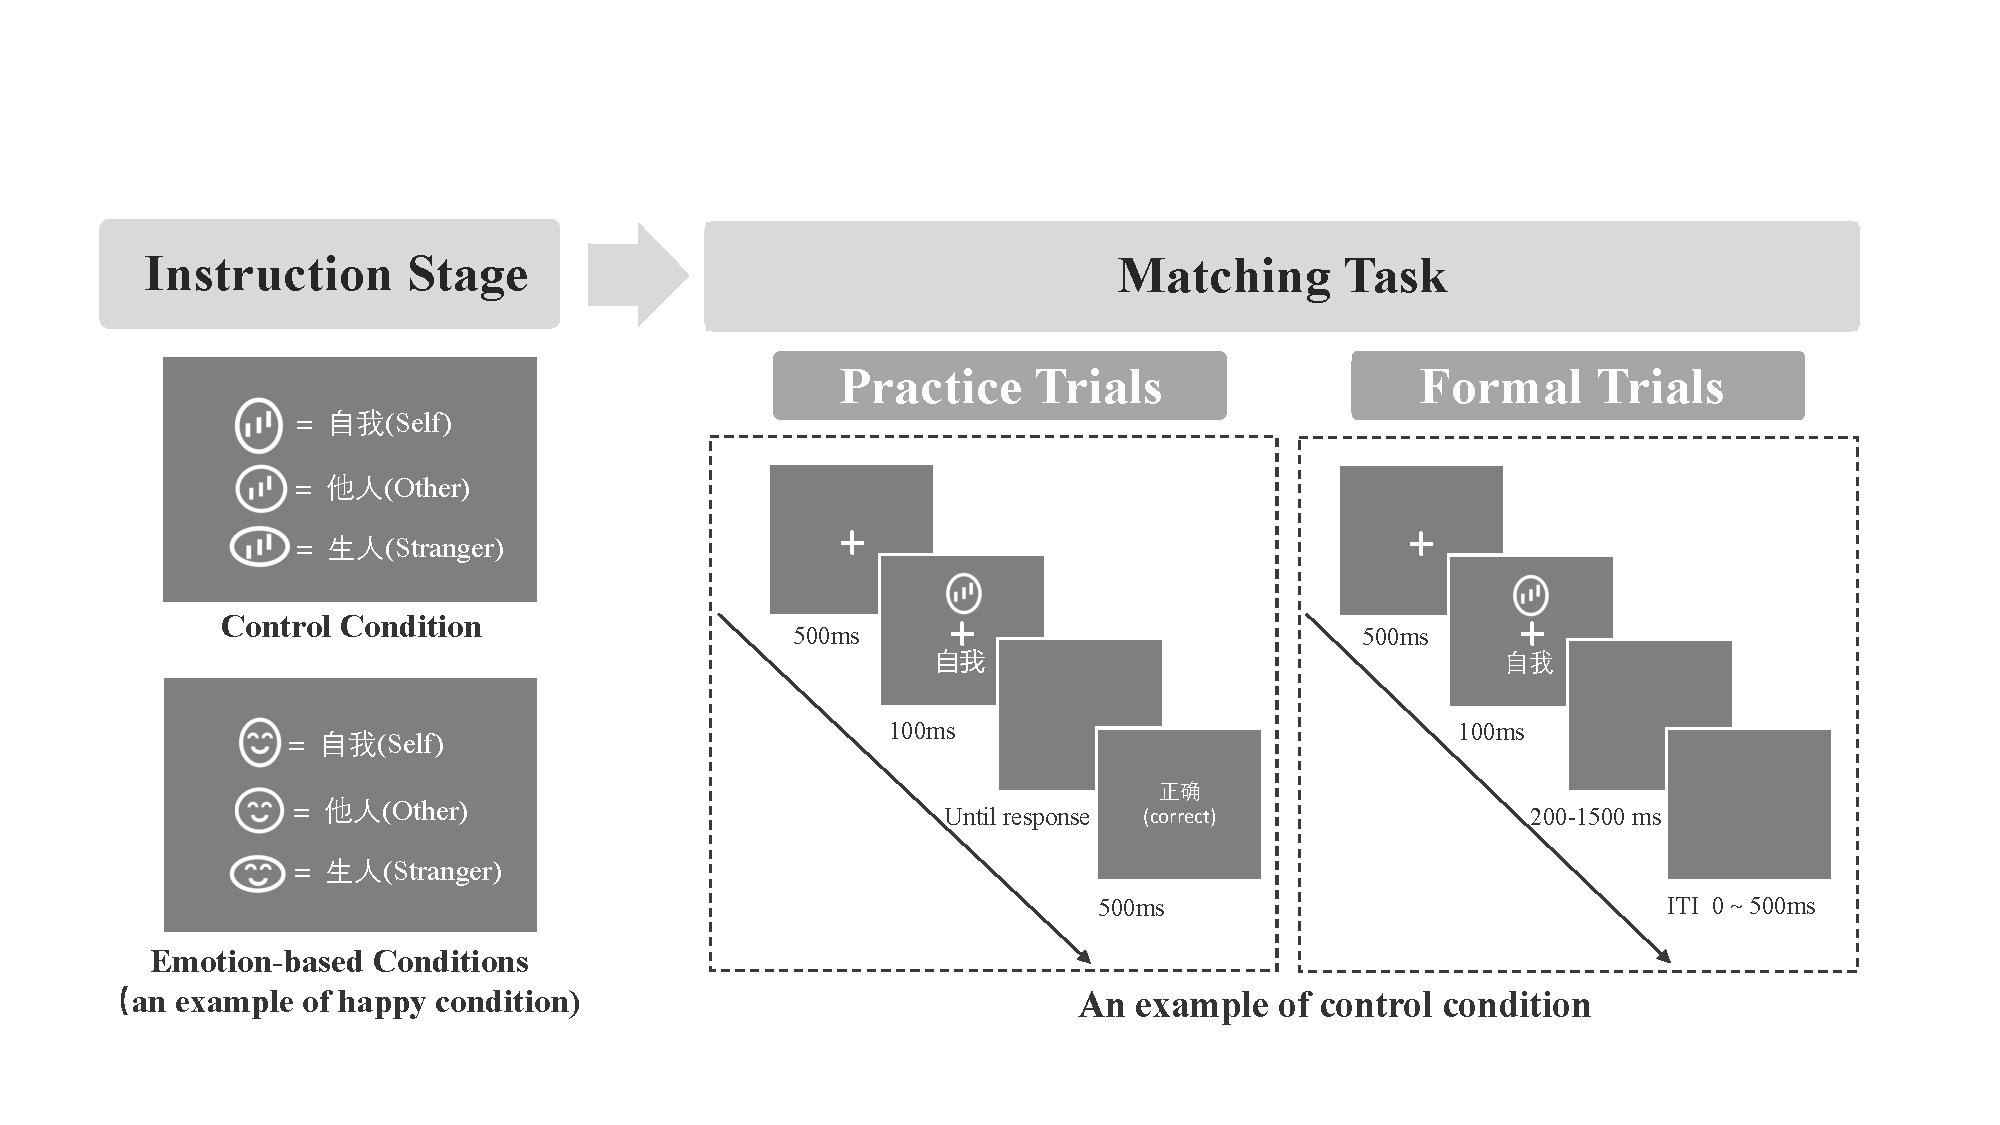
\includegraphics[width=1\textwidth]{./Figure/Fig1_Hu_pro.pdf}
	\caption[Procedure of the SPMT in Experiment B \parencite{hu2023data}]{	Procedure of the SPMT in Experiment B \parencite{hu2023data}. \textit{Note}: The labels and feedback appeared in Chinese in the experiment. In the associative learning task, the matched associations of shapes and labels was counterbalanced between participants. Timely feedback was not provided in formal trials.}
	\label{fig:Hu_SPMT_procedure}
\end{figure}

\subsubsection{Procedure}\label{subsec:procedure}

The experiment was finished individually in a dimly lighted room. Stimuli were presented and responses were collected using E-Prime 2.0 on PC. The monitor was at 1024 × 768 resolution with 100 Hz refresh rate.

The experiment has two phases (see Fig.  \ref{fig:Hu_SPMT_procedure}). Following \textcite{sui2012perceptual}, the first phase comprised a instruction stage in which participants were required to associate geometric shapes with labels. The shapes were not presented at this stage. The instruction stage lasted for approximately 60 seconds and shape-target associations were counterbalanced across the sample. Next, participants performed a matching task. At the start of each trial, a fixation cross was first displayed in the center of the screen for 500 ms. Then, a shape–label pairing as well as the fixation cross was presented for 100ms, respectively. The next frame showed a blank screen for 1500 ms, or until a response was made. Participants were asked to determine whether the shape was appropriately matched to the label by pressing one of the two response buttons as quickly and precisely as possible within this timeframe. 

The participants needed to separately learn 4 sets of association between shapes and labels. The associations contained 1 control condition and 3 sets of emotion-based condition. In the control condition, participants learned the association between 3 geometric shapes (circle, horizontal ellipse and vertical ellipse) and three labels (Self, Friend, Stranger). In each of the emotion-based condition, participants would see facial expressions (happy, sad, neutral) appear on the circle, horizontal ellipse and vertical ellipse (see Fig. \ref{fig:Hu_SPMT_procedure}). In each condition, before commencing the formal experimental trials, participants underwent a training session comprising 24 practice trials. After the practice trials, each participant completed 6 blocks of 60 trials in the task. There were six types of shape-label associations: Matching (Matching / Non-matching) x Shape (Self, Friend, Stranger) associations, with 60 trials for each association. Participants took a short break (up to 60 seconds) after each block. Each participant was required to repeat the experiment six times, with a one-week gap between each wave of experiments.

\subsection{Parameter Recovery Results for Package Comparison }\label{sec:ParameterRecovery}

We chose not to utilize the HDDM package \parencite{wiecki2013hddm} since the computation process was significantly time-consuming, necessitating high computational resources and leading to prolonged overall analysis time. Instead, we performed a package comparison by generating 100 datasets using the HDDM package in Python, in order to identify the most appropriate package for our analysis. These datasets were specifically configured with parameters $a = 2$, $t = 0.3$, $v = 1$, and $z = 0.7$. 

Subsequently, we utilized three widely used DDM packages in R, namely RWiener \parencite{viechtbauer2010conducting}, hausekeep \parencite{Lin2019how}, and FastDMinR \parencite{voss2007fast}, to compute parameter estimates for these generated datasets. The evaluation process involved comparing the computed values obtained from the R packages with the set parameters. If the computed values from the R packages were found to be closer to the set values, it signified that the respective R package provided more accurate parameter estimation for the DDM.

Fig. \ref{fig:DDM_comparision} presents the results of the package comparison. The estimated drift rate (\textit{v}) obtained from RWiener was 1.01, with a 95\% confidence interval of [.98, 1.03], which closely aligned with our pre-defined values. Similarly, the estimated starting point (\textit{z}) is 0.77, with a 95\% confidence interval of [.76, .78], also very close to our pre-defined value. On the contrary, the parameters calculated using other packages either showed high inaccuracies, excessively wide confidence intervals, or required extended computation times. As a result, we have opted to utilize RWiener for our calculations. It struck a favorable balance between accuracy, confidence interval width, and computational efficiency, making it the most suitable choice for our analysis.
\clearpage

\begin{figure}[!ht]
	\centering
	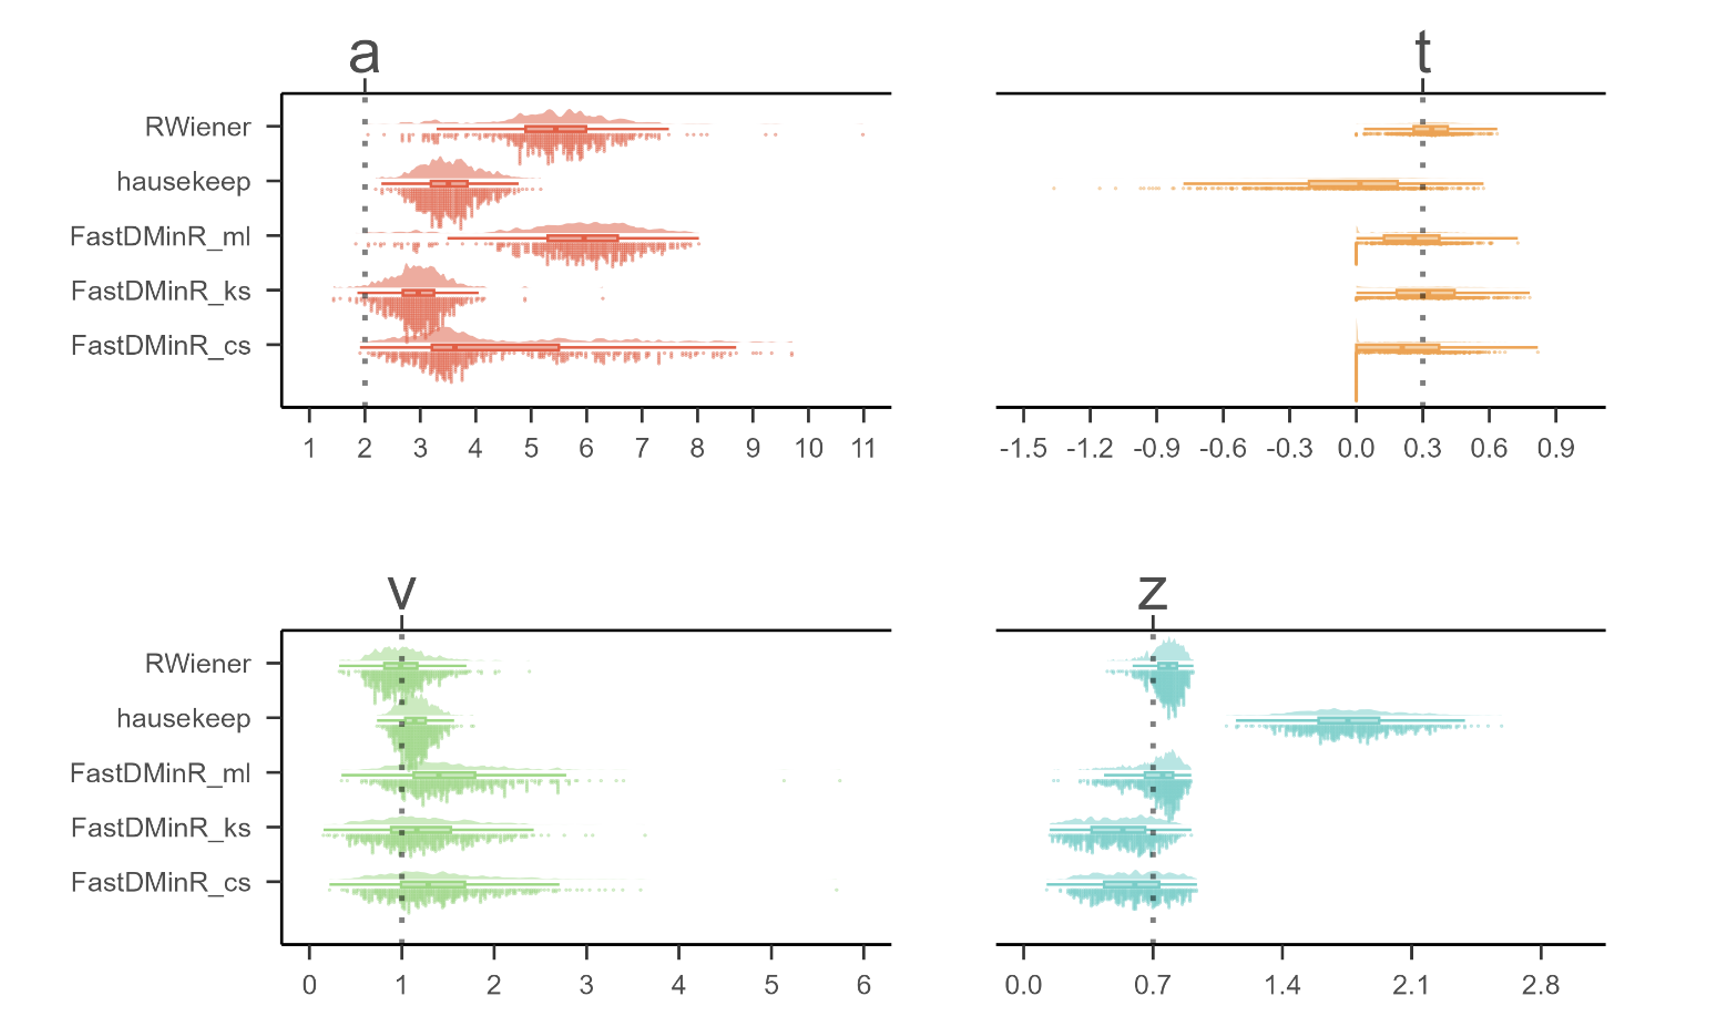
\includegraphics[width=1\textwidth]{./Figure/Fig2_DDM_comparision.png}
	\caption[DDM Packages Comparison]{DDM Packages Comparison. \textit{Note}: The parameters of interest in the Drift-Diffusion Model (DDM) are represented as follows: ``\textit{a}" denotes the threshold parameter, ``\textit{t}" represents the non-decision time, ``\textit{v}" indicates the drift rate, and ``\textit{z}" corresponds to the starting point. The y-axis of the graph displays the estimation of these DDM parameters using three different R packages: ``RWiener," ``hausekeep," and ``FastDMinR." In total, there are five methods for estimating DDM parameters, with three methods originating from the ``FastDMinR" package. On the x-axis, the values of the estimated parameters are plotted. The dashed line on the graph indicates the true value of the parameter being estimated.
	}\label{fig:DDM_comparision}
\end{figure}


\section{Supplementary Results}\label{Results}

\subsection{Group Level SPE for Other Measures}\label{sec:meta}
We conducted a meta-analysis of all the 6 indicators of SPE. The Forest Plots were presented in Fig. \ref{fig:Meta_Result}. 
\clearpage
\begin{figure}[!ht]
	\centering
	\includegraphics[width=1\textwidth]{./Figure/Fig6_Forest_Supp.png}
	\caption[Forest Plot for SPE Measures]{Forest Plot for SPE Measures. \textit{Note}: Fig (a)-(f) represent the forest plots corresponding to RT, ACC, $d'$, $\eta$, \textit{v}, and \textit{z} under the condition where Target is Close. Fig (g)-(l) represent the forest plots corresponding to $d'$, $\eta$, \textit{v}, and \textit{z} under the condition where Target is Stranger.
	}\label{fig:Meta_Result}
\end{figure}
\clearpage

Due to the limited availability of papers on ``Celebrity“ and ``Nonperson”, we were unable to perform a meta-analysis on these baselines. Instead, we conducted paired-sample t-tests comparing self and baseline conditions. Hedges' $g$ was calculated and the results were presented in Table. \ref{table:t-testresult}. Considering there is only one paper available for these baselines, it is advisable to approach these results with caution.


\renewcommand{\thetable}{S\arabic{table}}

\begin{table}[!ht]
	\caption{T-test Results of SPE Measures in SPMT}\label{table:t-testresult}
	\label{table:Meta}%
	\begin{tabular}{@{}lcccccc@{}}
		\toprule
		Baseline & Indicators & Hedges’ $g[95\% \text{CI}]$& $t$ & $df$ & $p$\\
		\midrule
		Celebrity &  $\text{RT}$& $1.76\ [1.11, 2.41]$& 5.28& 24 & $<.001$\\
		&  $\text{ACC}$ & $2.08\ [1.39, 2.77]$& 5.93&24&$<.001$ \\
		&  $d'$ &$1.41\ [.79, 2.03] $&4.45&24&$<.001$ \\
		&  $\eta$ & $2.70\ [1.93, 3.46]$&6.90&24&$<.001$ \\
		&  \textit{v} &$1.45\ [.83, 2.08]$ &4.57&24&$<.001$ \\
		&  \textit{z} & $.05\ [-.50, .61]$&0.19&24&.85 \\
		
		NonPerson &  $\text{RT}$ &$-.13\ [-.62, .36]$ &-.51&31&.61 \\
		&  $\text{ACC}$ &$.02\ [-.47, .51]$ &.07&31&.95\\
		&  $d'$ & $.17\ [-.32, .66]$ &.68&31&.50\\
		&  $\eta$ & $-.09\ [-.58, .40]$&-.36&31&.72 \\
		&  \textit{v} & $.33\ [-.16, .83]$&1.32&31&.19\\
		&  \textit{z} & $-.45\ [-.95, .04]]$&-1.79&31&.07 \\
		\botrule
	\end{tabular}
\end{table}

\subsection{Split-Half Reliability Using Four Splitting Approaches}\label{sec:SHR}

In this section, we presented the Split-Half Reliability (SHR) results for the SPE measures using four split-half methods: Monte Carlo, first-second, odd-even, and permutated. We also included  the drift rate (\textit{v}) and starting point (\textit{z}) estimated from the ``hausekeep" package in the analysis. However, it's important to highlight that the estimation of parameter ``\textit{a}" in ``hausekeep" significantly deviates from the HDDM approach, primarily because of its assumption that $z = a / 2$ (refer to Fig. \ref{fig:DDM_comparision}). As a result, we have chosen not to include the results obtained from this package in the main text. Nevertheless, we presented them here for reference and transparency. Please refer to Fig. \ref{fig:SHR_Result} for the visual representation of the results.
\clearpage

\begin{figure}[ht]
	\centering
	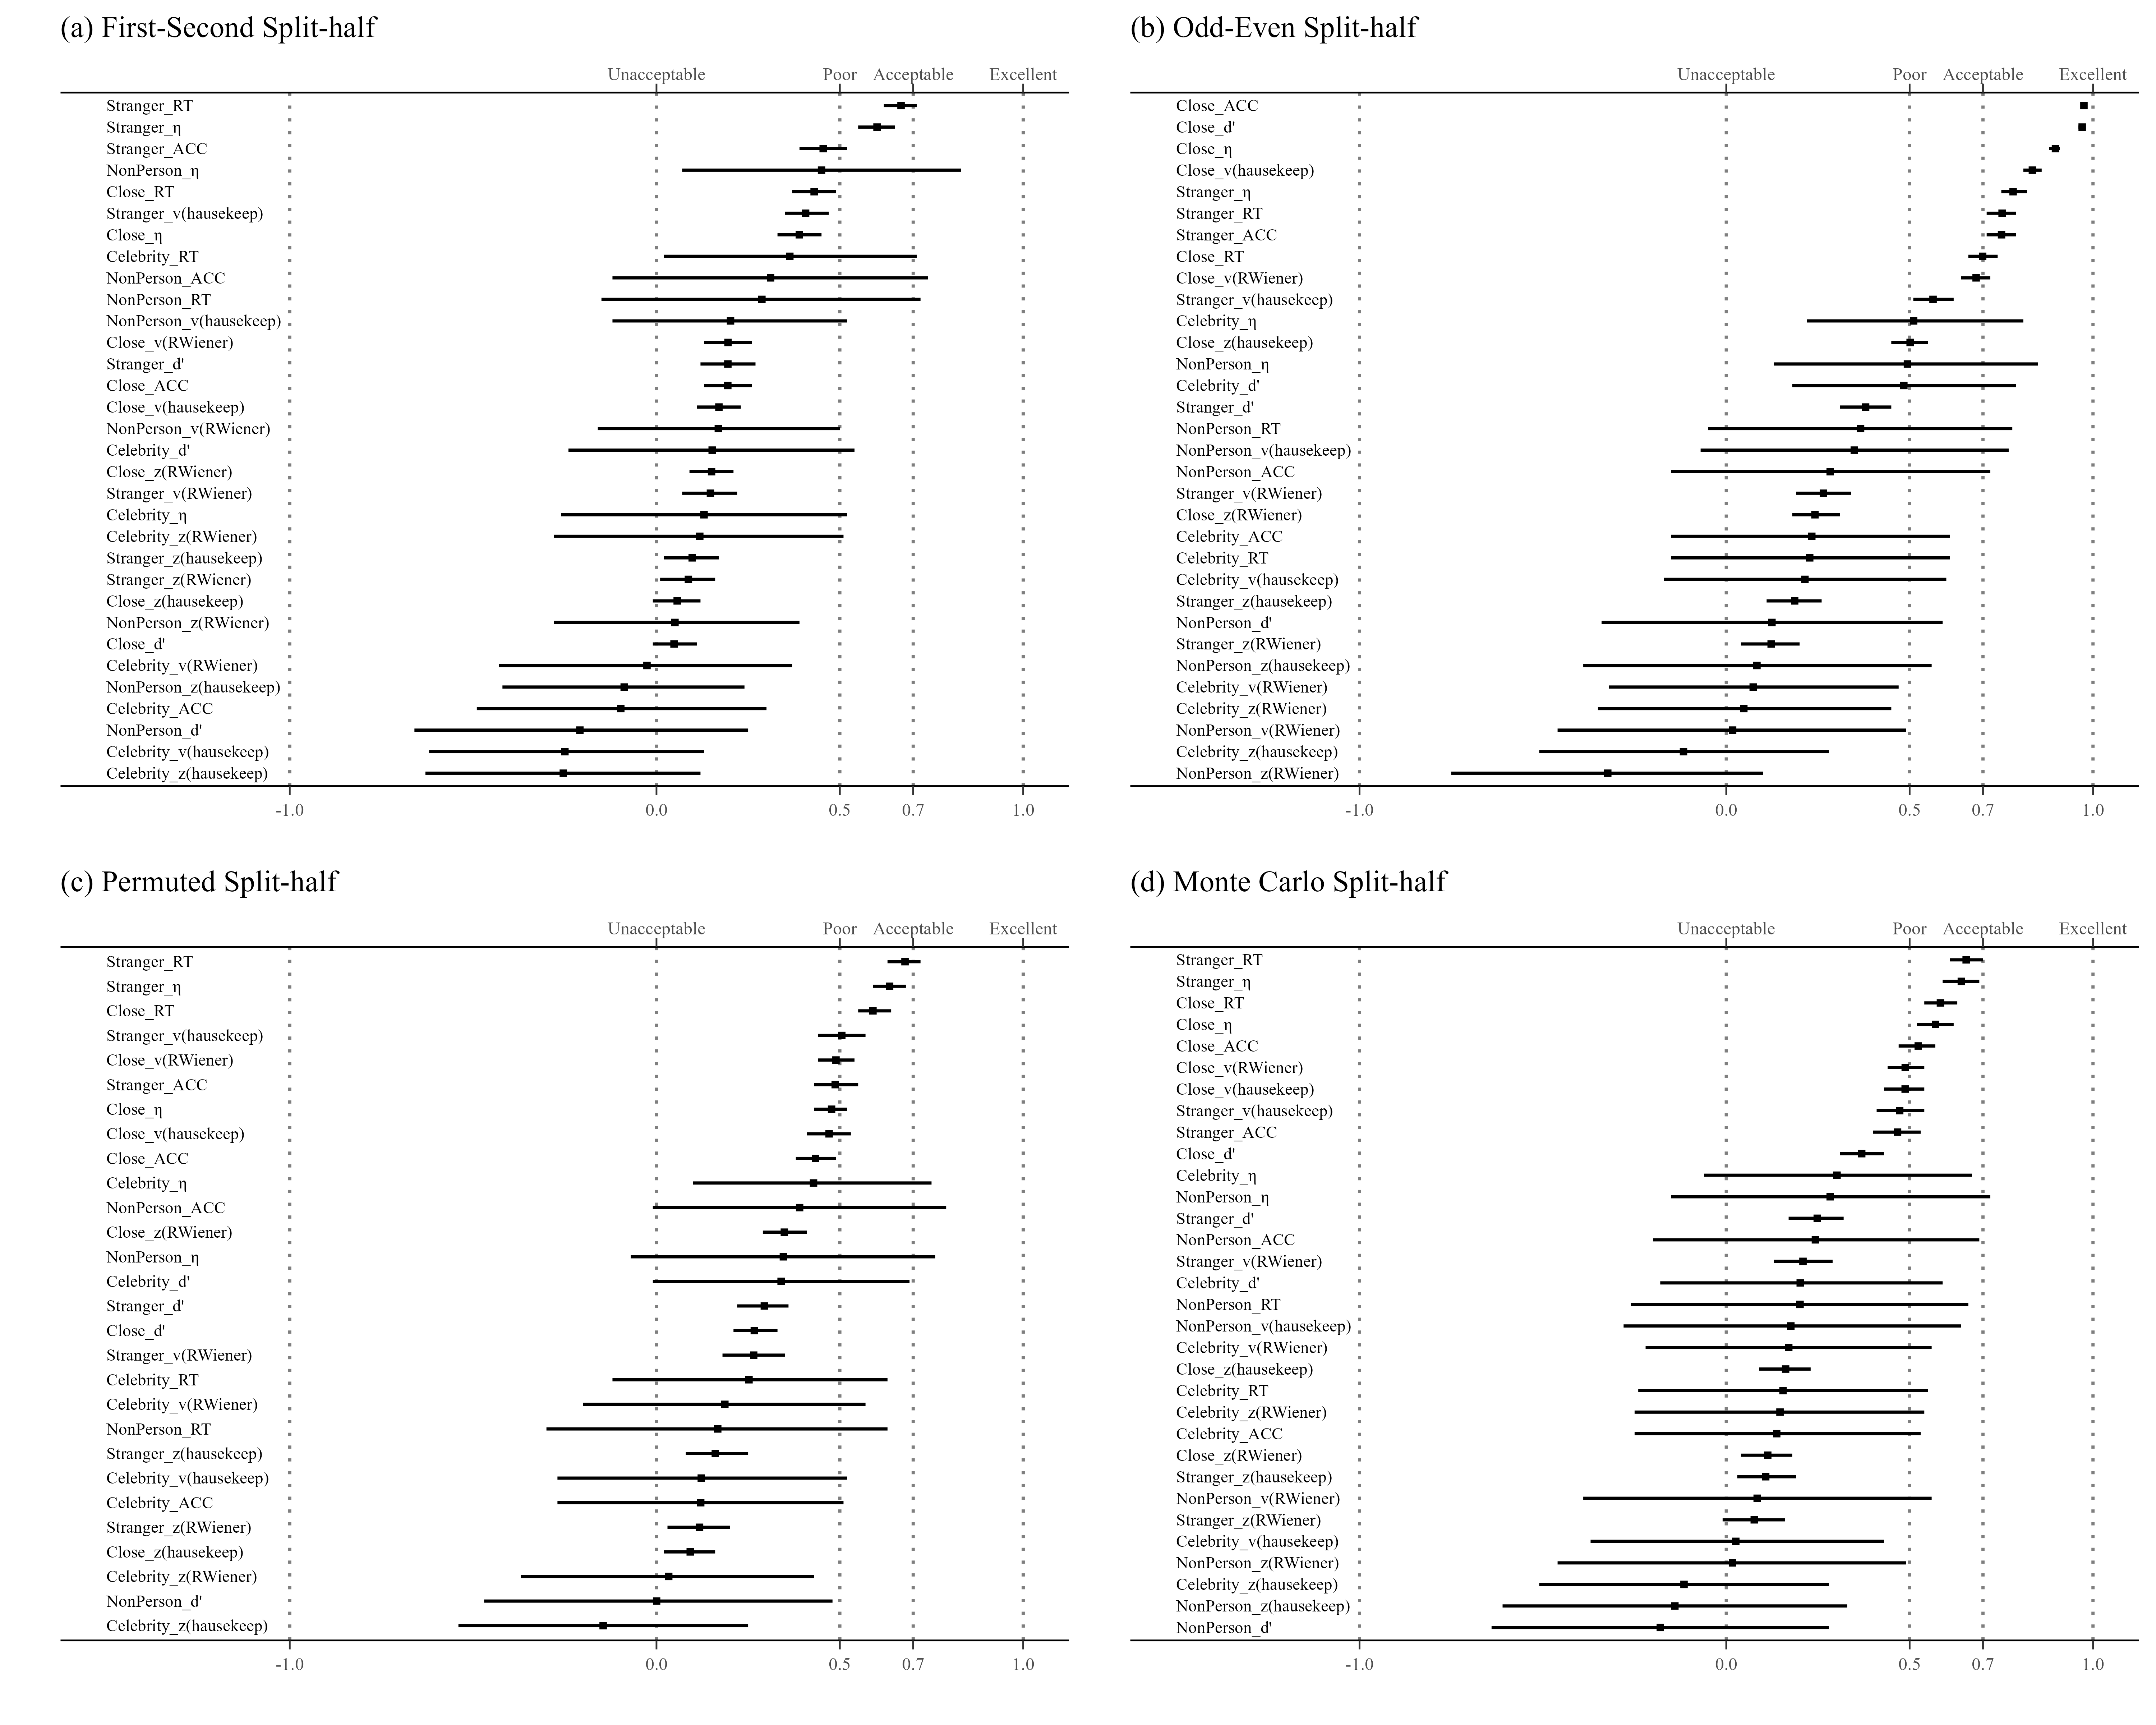
\includegraphics[width=1\textwidth]{./Figure/Fig3_SHR.png}
	\caption[Results of SHR Using Four Split-half Methods]{Results of SHR Using Four Split-half Methods. (a) Results of SHR using First-Second Split-half Methods; (b) Results of SHR using Odd-Even Split-half Methods; (c) Results of SHR using Permuted Split-half Methods; (d) Results of SHR using Monte Carlo Split-half Methods. \textit{Note}: The vertical axis of the graph listed 32 different SPE measures, combining six indicators (RT, ACC, $d’$, $\eta$, \textit{v}, \textit{z}) and four baseline conditions (close other, stranger, celebrity, and non-person). The \textit{v} and \textit{z} implemented using the ``hausekeep" package were also included. The weighted average split-half reliability and 95\% confidence intervals are shown by points and lines. The figure is divided into separate facets arranged from left to right, each representing weighted average split-half reliability calculated using three distinct methods: first-second, odd-even, and permuted. 
	}\label{fig:SHR_Result}
\end{figure}


It's evident that the results pattern from the permuted split-half methods and first-second split-half methods closely resembled the Monte Carlo method's outcomes. The top four split-half reliabilities, ranked highest, were as follows: Reaction Time (RT) with the "Stranger" contrast, Efficiency ($\eta$) with the ``Stranger" contrast, RT with the "Close other" contrast, $\eta$ with the ``Self vs Close" contrast. However, the results obtained from the odd-even split-half method were notably different from the other three methods. We hypothesize that this discrepancy may be attributed to the odd-even method's sensitivity to temporal dependencies, which could have been influenced by the inherent sequential nature of responses in the SPMT. Further investigation into the presence and impact of serial dependency in the data would be valuable to better understand the observed variations in the split-half reliabilities among the different methods.

\subsection{ICCs for SPE Measures Using Another Dataset}\label{sec:ICC}

In Fig. \ref{fig:ICC_Result}, we presented the results of the Intraclass Correlation Coefficients (ICC2) for the SPE measures, where drift rate (\textit{v}) and starting point (\textit{z}) estimated from the ``hausekeep" package were also included. In Fig. \ref{fig:ICC_Result}(b), we extended our exploration of ICC2 to include the SPE measures from one additional dataset. However, the SPMT used in this dataset deviated quite strongly from the original SPMT paradigm. Due to these significant differences, ICC2 obtained from this dataset may reflect variations introduced by the modified SPMT rather than directly comparable results to the original paradigm.

\begin{figure}[!ht]
	\centering
	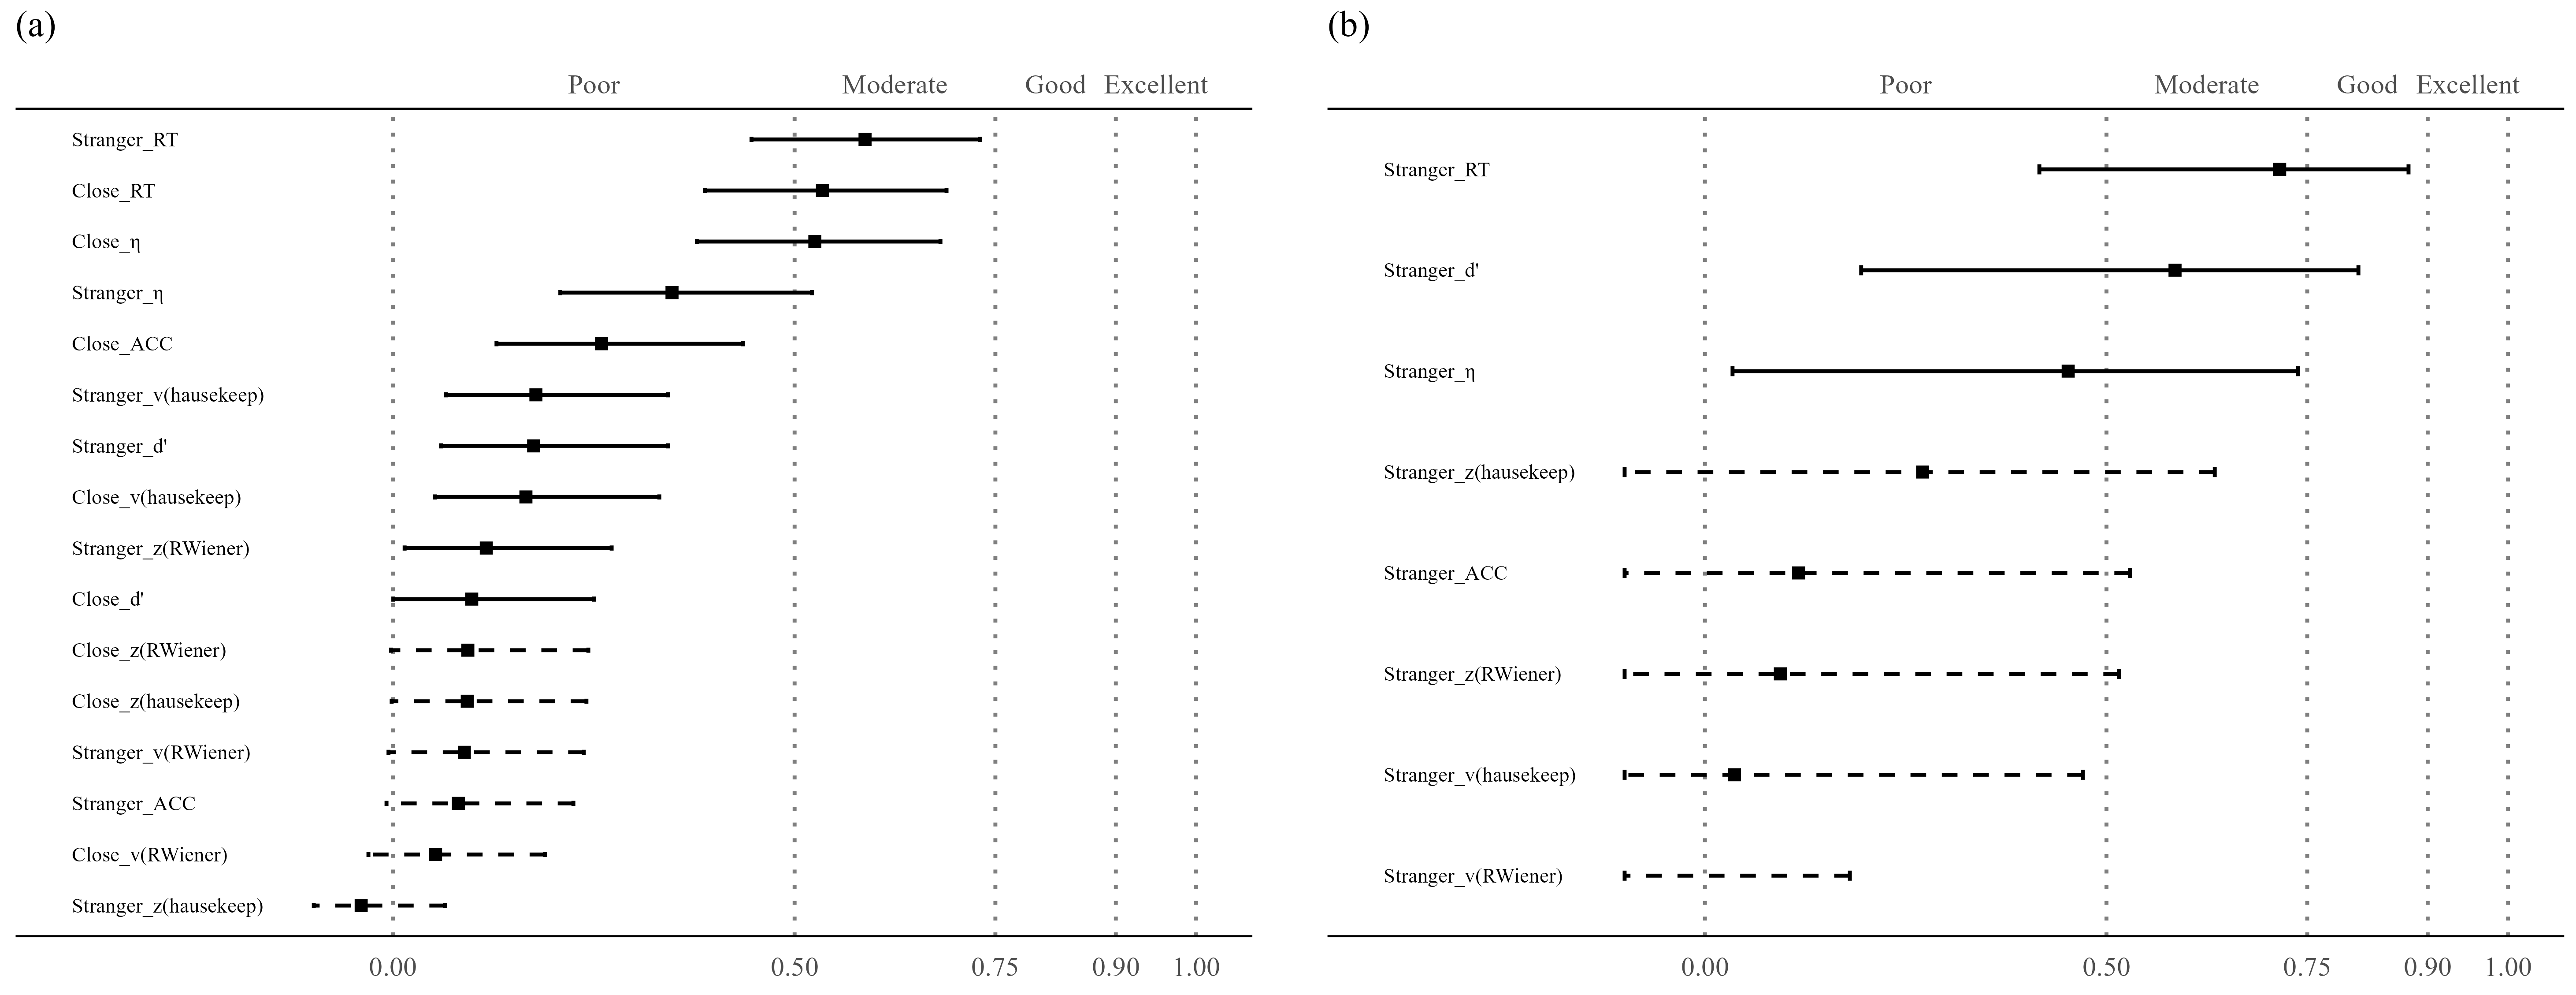
\includegraphics[width=1\textwidth]{./Figure/Fig4_ICC.png}
	\caption[ICCs for SPE Measures Using \textcite{hu2023data} and Another Dataset]{ICCs for SPE Measures Using \textcite{hu2023data} and Another Dataset. (a) ICC2 for SPE measures using \textcite{hu2023data}; (b) ICC2 for SPE measures using an additional dataset.  \textit{Note}: The vertical axis of the graph illustrates eight distinct indicators, which includes two additional indices from the DDM, implemented using the ``hausekeep" package. The line and dots on the graph represent the value of ICC2, along with their corresponding 95\% confidence intervals. The dashed line indicates that the confidence interval for that point estimate extends beyond the range of our coordinate axes (0, 1).
	}\label{fig:ICC_Result}
\end{figure}

Since the original design of \textcite{hu2023data} incorporated measures from the Beck Depression Inventory-II (BDI-II) \parencite{wang2011reliability}. Thus, in Fig. \ref{fig:BDI_cov_Result}, we incorporated the BDI-II scores of individual participants as covariates when calculating ICC2. Notably, even after accounting for these BDI scores as covariates, we observed consistent ICC2 values both before and after this adjustment.
\clearpage

\begin{figure}[!ht]
	\centering
	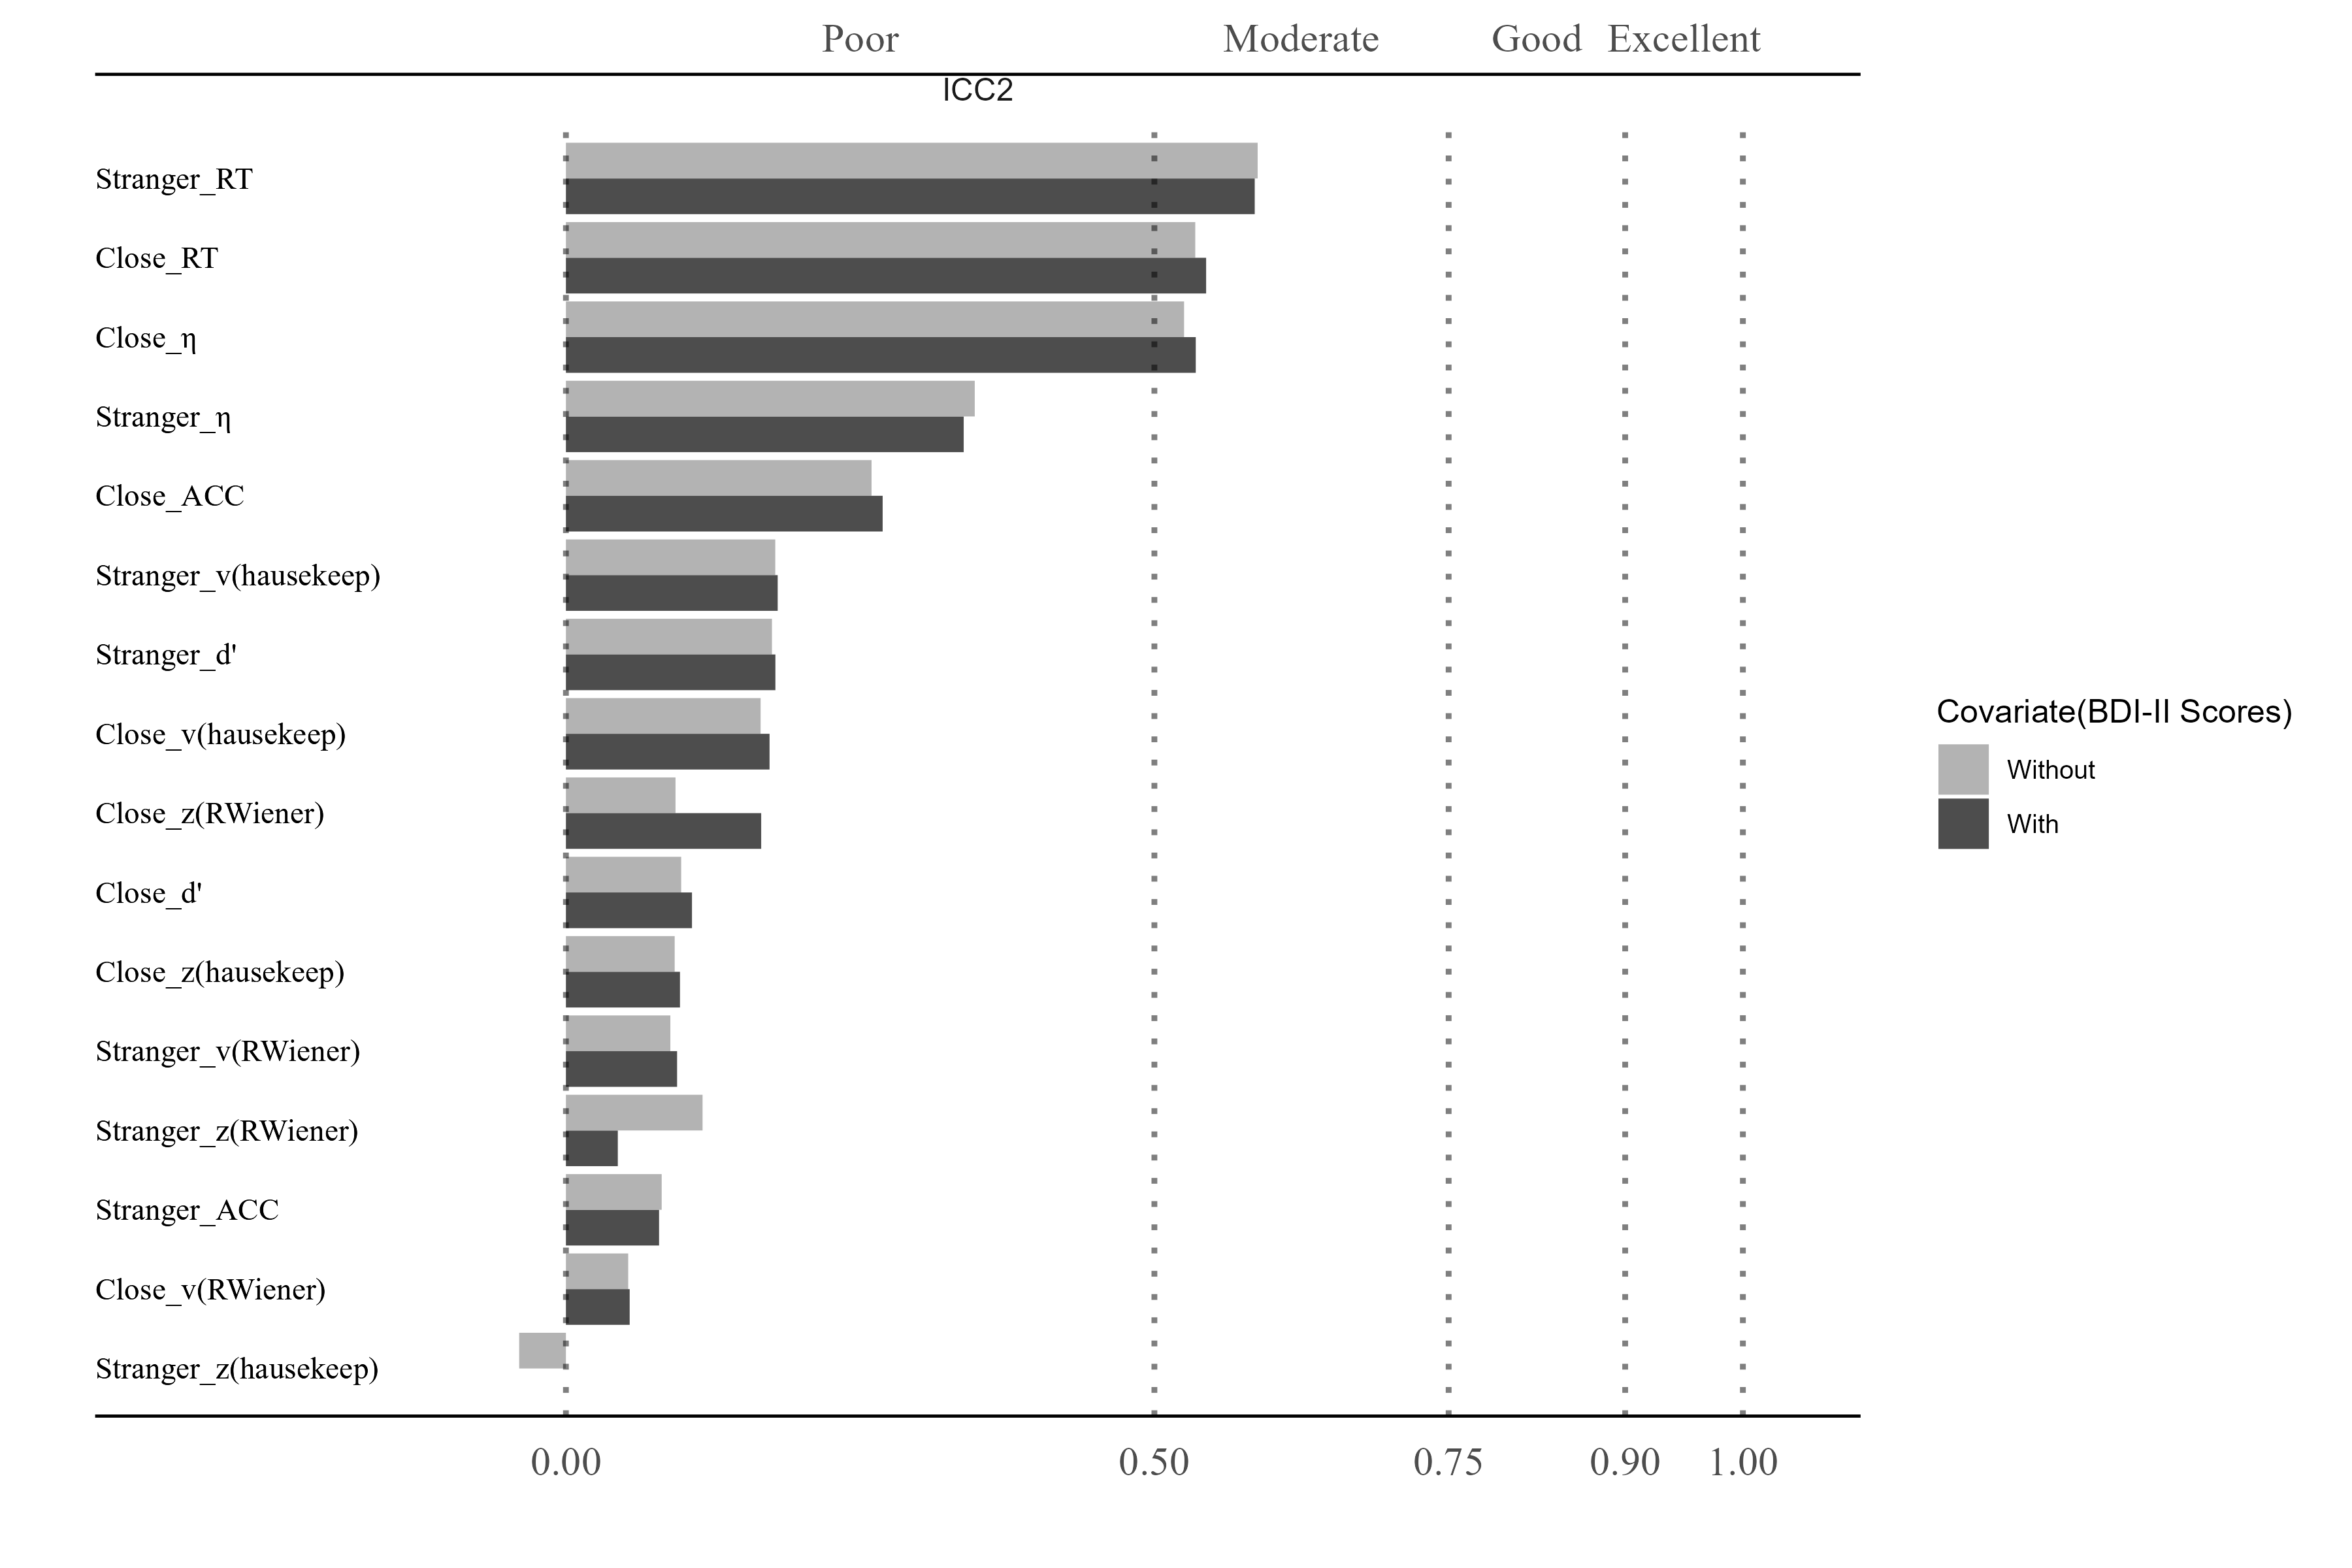
\includegraphics[width=1.1\textwidth]{./Figure/Fig5_BDI_cov.png}
	\caption[ICC2 for SPE Measures Using \textcite{hu2023data} with Covariant (BDI-II Scores)]{ICC2 for SPE Measures Using \textcite{hu2023data} with Covariant (BDI-II Scores).  \textit{Note}: The vertical axis of the graph illustrates eight distinct indicators, which includes two additional indices from the DDM, implemented using the ``hausekeep" package. The bar on the graph represent the value of ICC2.
	}\label{fig:BDI_cov_Result}
\end{figure}


\subsection{Exploratory Analysis}\label{sec:Exploratory}

In this section, we presented the results of the exploratory analysis of the current study. Our focus was on performing a correlation analysis that assessed the relationship between the number of trials and two key factors: Monte Carlo split-half reliability and effect size (Hedges’ \textit{g}). We also examine the relationship between Monte Carlo split-half reliability and effect size (Hedges’ \textit{g}).

We found significant correlations between trial numbers and Monte Carlo split-half reliability for some indicators, such as Reaction Time and Efficiency (see Fig. \ref{fig:R_nTrial}) . However, for indicators like $d'$ and \textit{v}, the correlation with trial numbers was relatively weak. Moreover, we could observe that the SPMT paradigm requires approximately 80 trials to achieve a Monte Carlo split-half reliability of 0.8 for the SPE measure of RT under the ``Stranger' condition and around 120 trials under the ``Close' condition. Furthermore, achieving a Monte Carlo SHR of 0.8 of  the parameter \textit{v} may required more than 120 trials. On the other hand, attaining high Monte Carlo SHR values for the remaining three indicators, particularly for the \textit{z} parameter, remains challenging even with 150 or more trials.
\begin{figure}[!h]
	\centering
	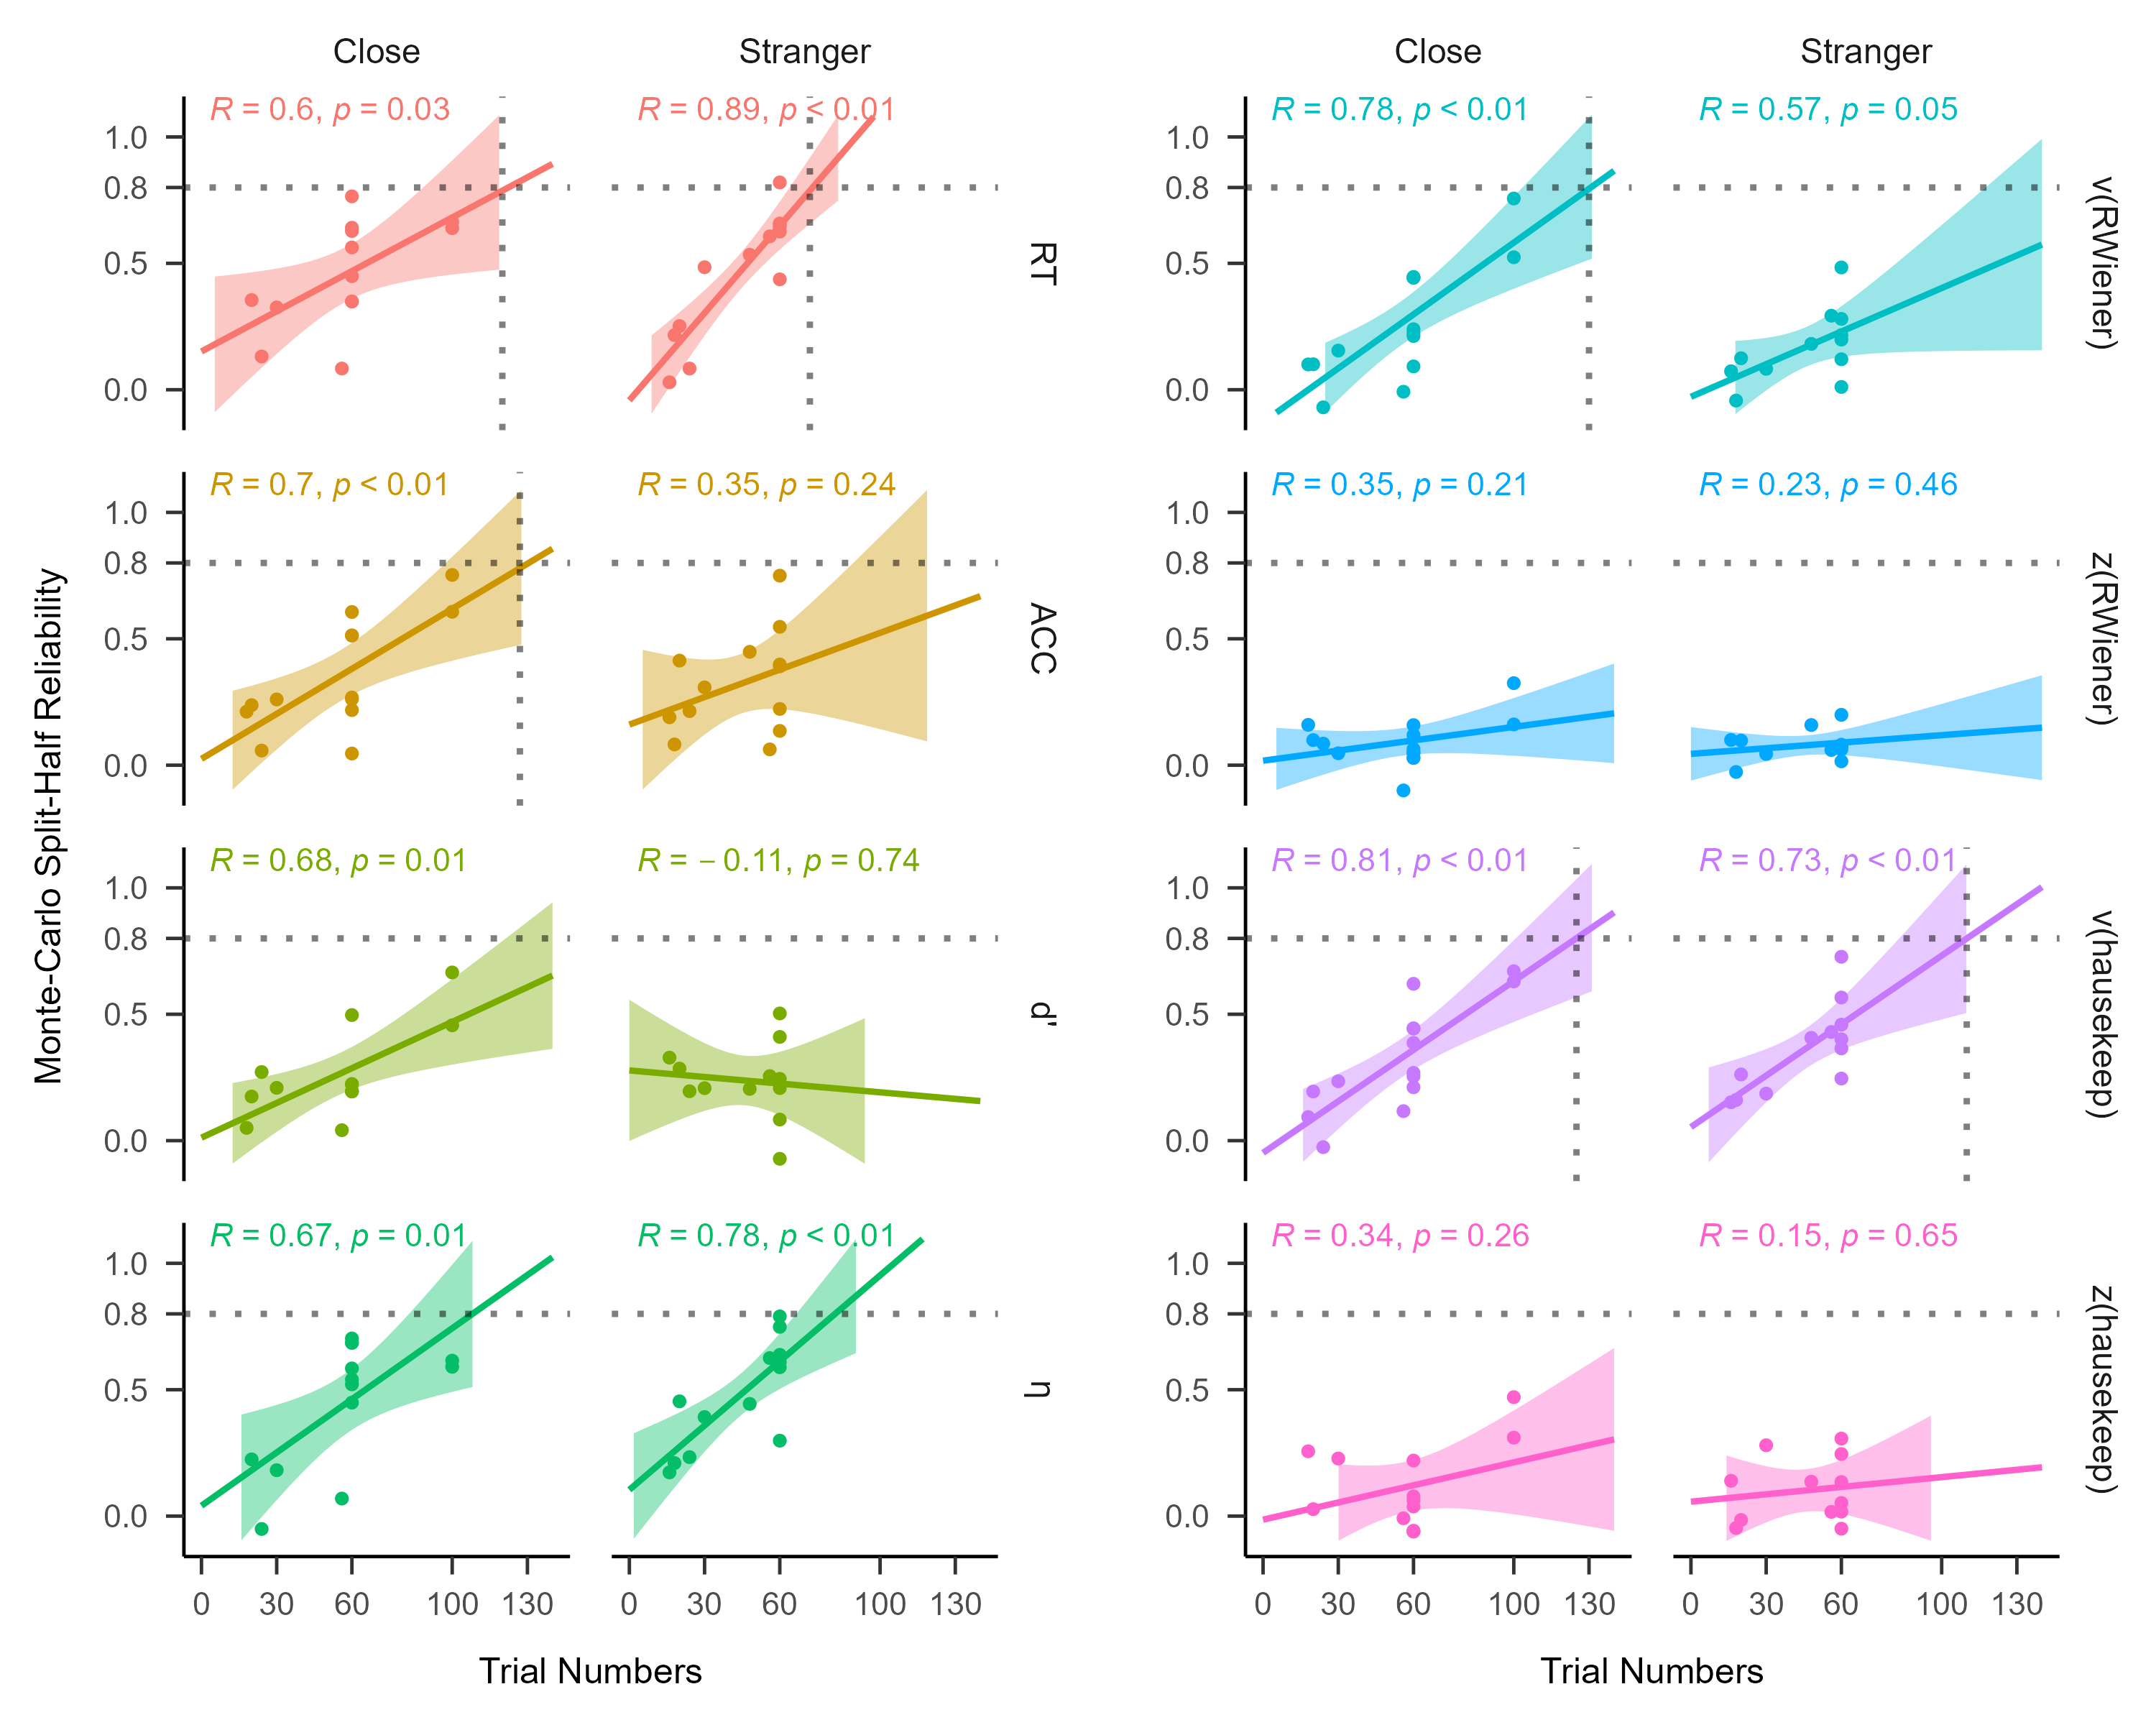
\includegraphics[width=1\textwidth]{./Figure/Fig7_r&Trial.png}
	\caption[Regression Analysis Between Monte Carlo SHR and Trial Numbers Using Different SPE Measures.]{Regression Analysis Between Monte Carlo SHR and Trial Numbers Using Different SPE Measures.  \textit{Note}: The vertical axis represents Monte-Carlo split-half reliability, and the horizontal axis represents the number of trials. Each facet represents one SPE measures.
	}\label{fig:R_nTrial}
\end{figure}
\clearpage

We also explored the correlation between split-half reliability and effect size (Hedges’ \textit{g}), as shown in Fig. \ref{fig:g_r}. Our exploratory analysis did not find a significant correlation among them. This result pattern was some how consistent with the reliability paradox \parencite{logie1996group,hedge2018reliability}, which suggested that robust experimental effects are not always associated with robust individual difference correlations.

\begin{figure}[!ht]
	\centering
	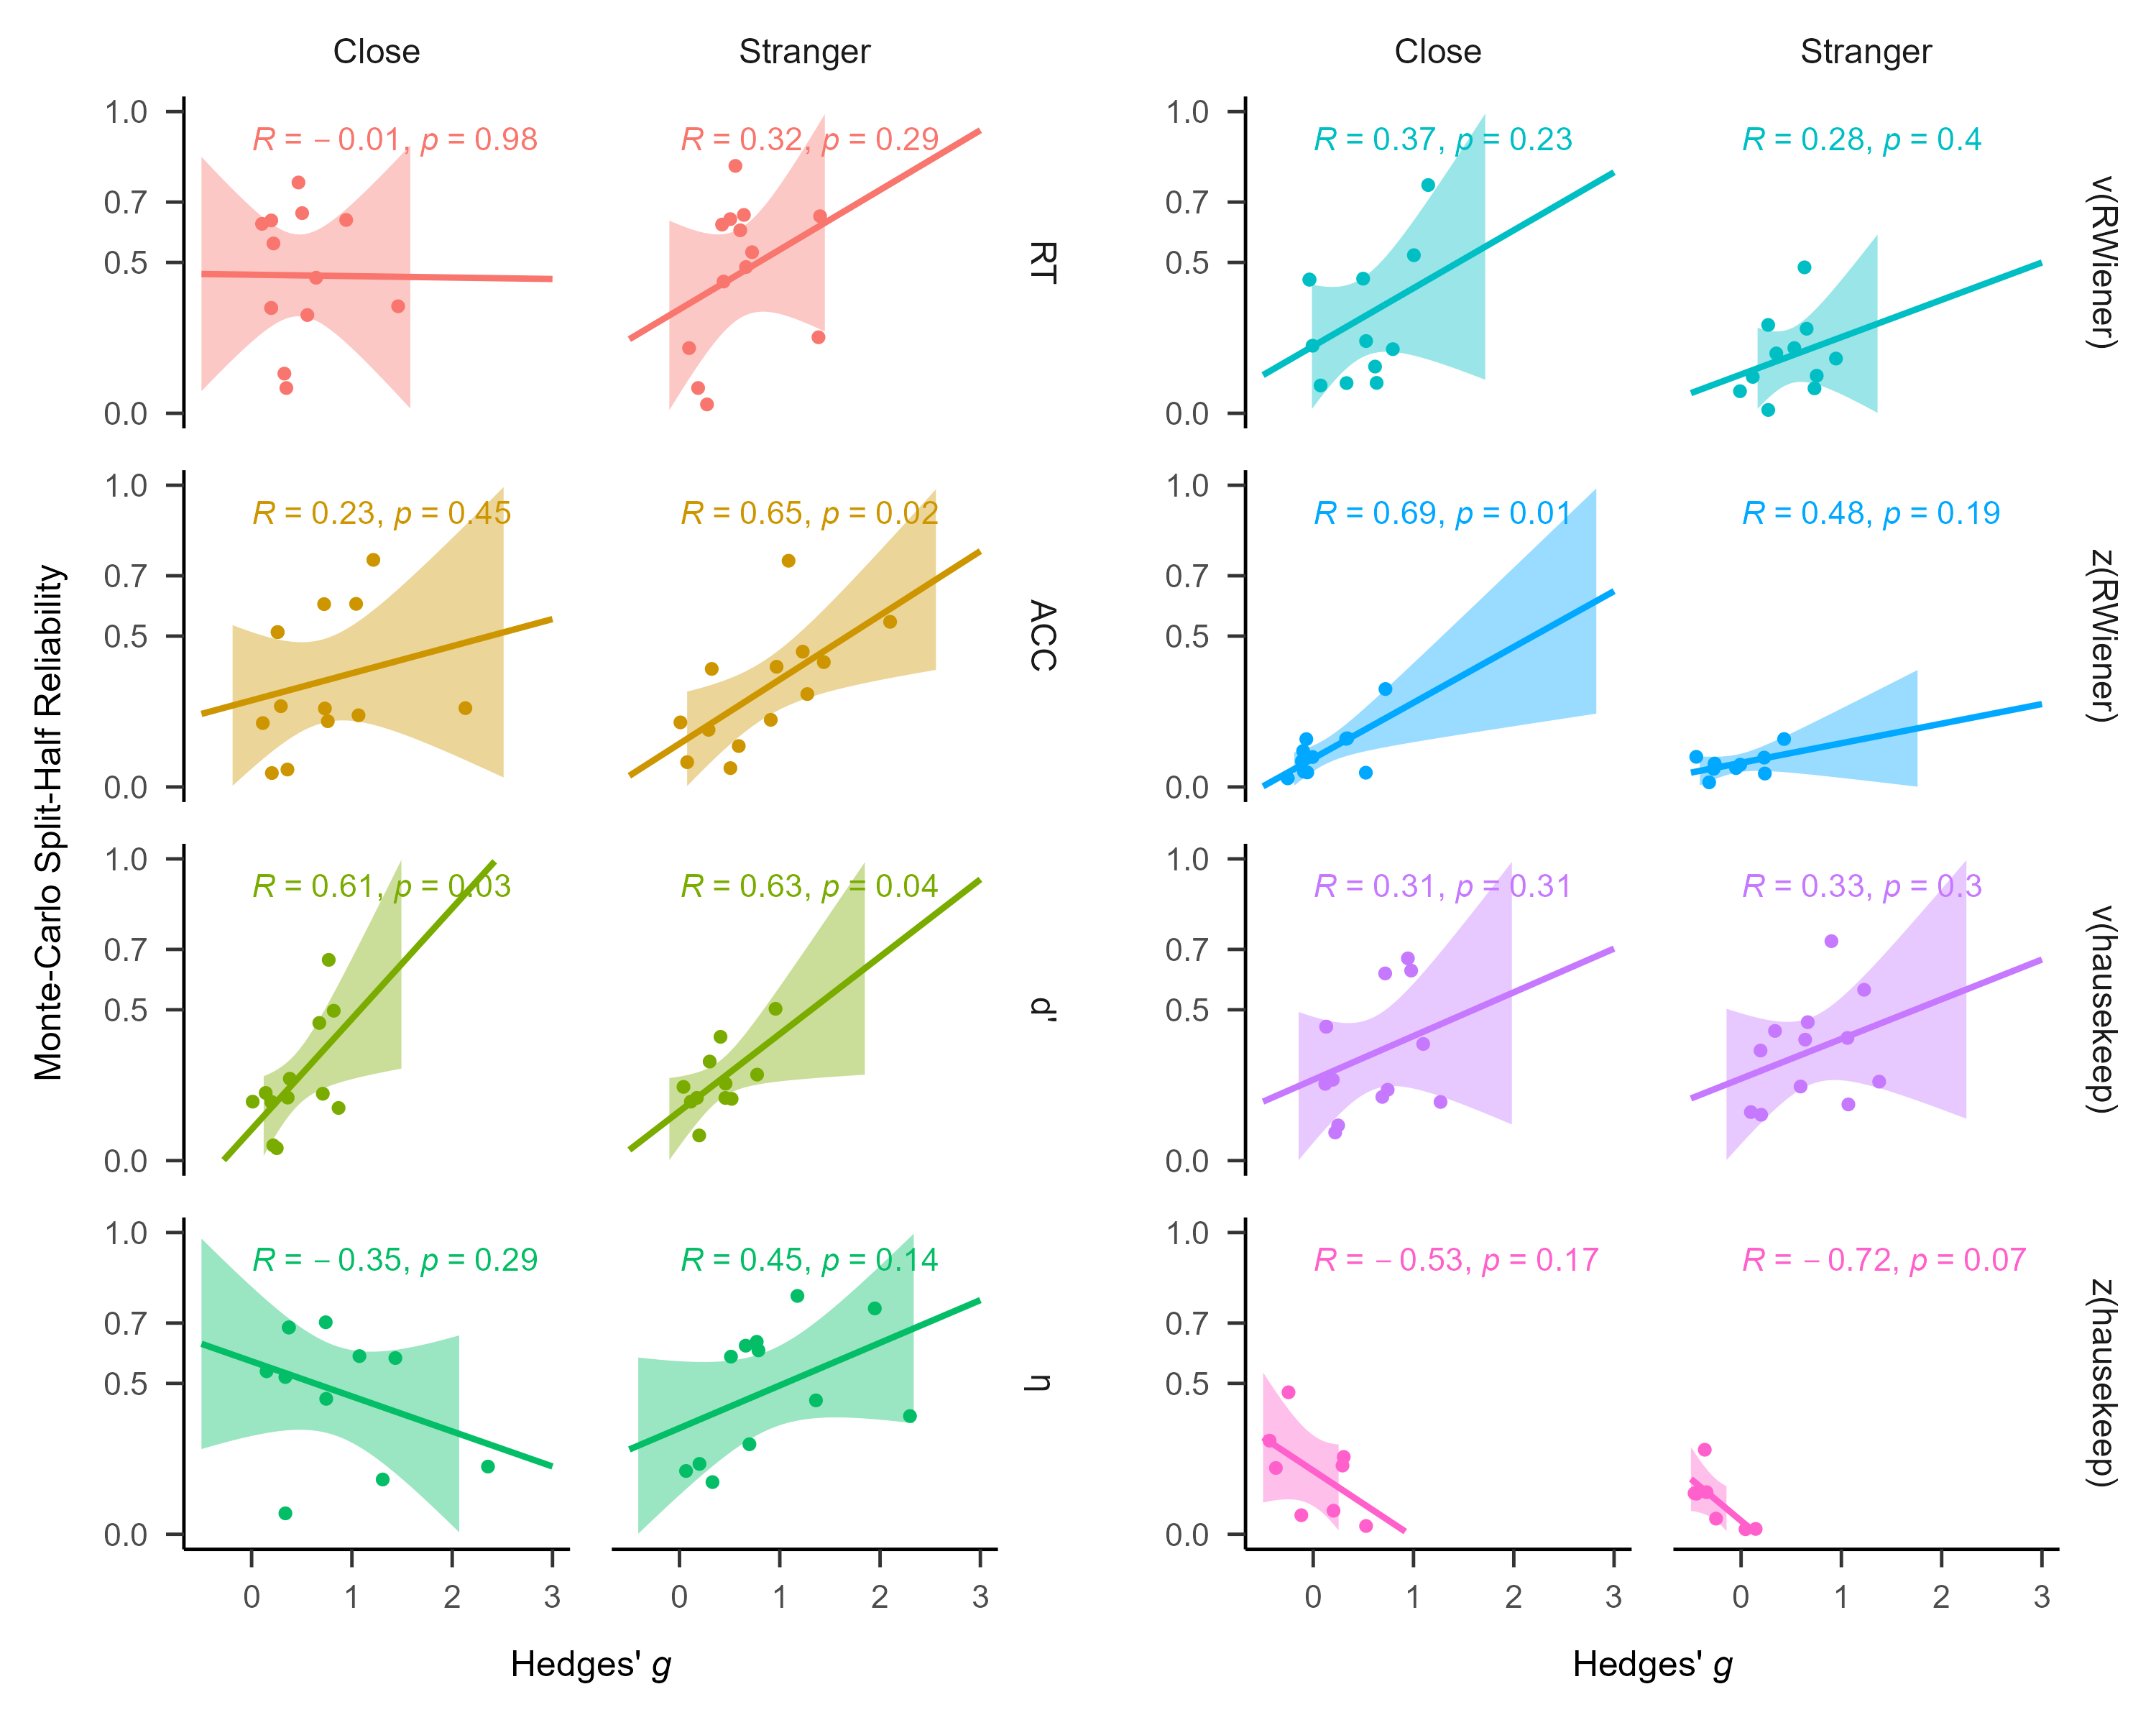
\includegraphics[width=1\textwidth]{./Figure/Fig8_yi&r.png}
	\caption[Regression Analysis Between Monte Carlo SHR and Effect Size (Hedges’ \textit{g}) Using Different SPE Measures]{Regression Analysis Between Monte Carlo SHR and Effect Size (Hedges’ \textit{g}) Using Different SPE Measures. \textit{Note}: The vertical axis represents Monte-Carlo split-half reliability, and the horizontal axis represents the effect size (Hedges’ g). Each facet represents one SPE measures.
	}\label{fig:g_r}
\end{figure}
\clearpage

Finally, we calculated the correlation coefficient between trial numbers and effect size (Hedges’ \textit{g}), as shown in Fig. \ref{fig:g_nTrial}. Similarly, no significant correlation was found.

\begin{figure}[!ht]
	\centering
	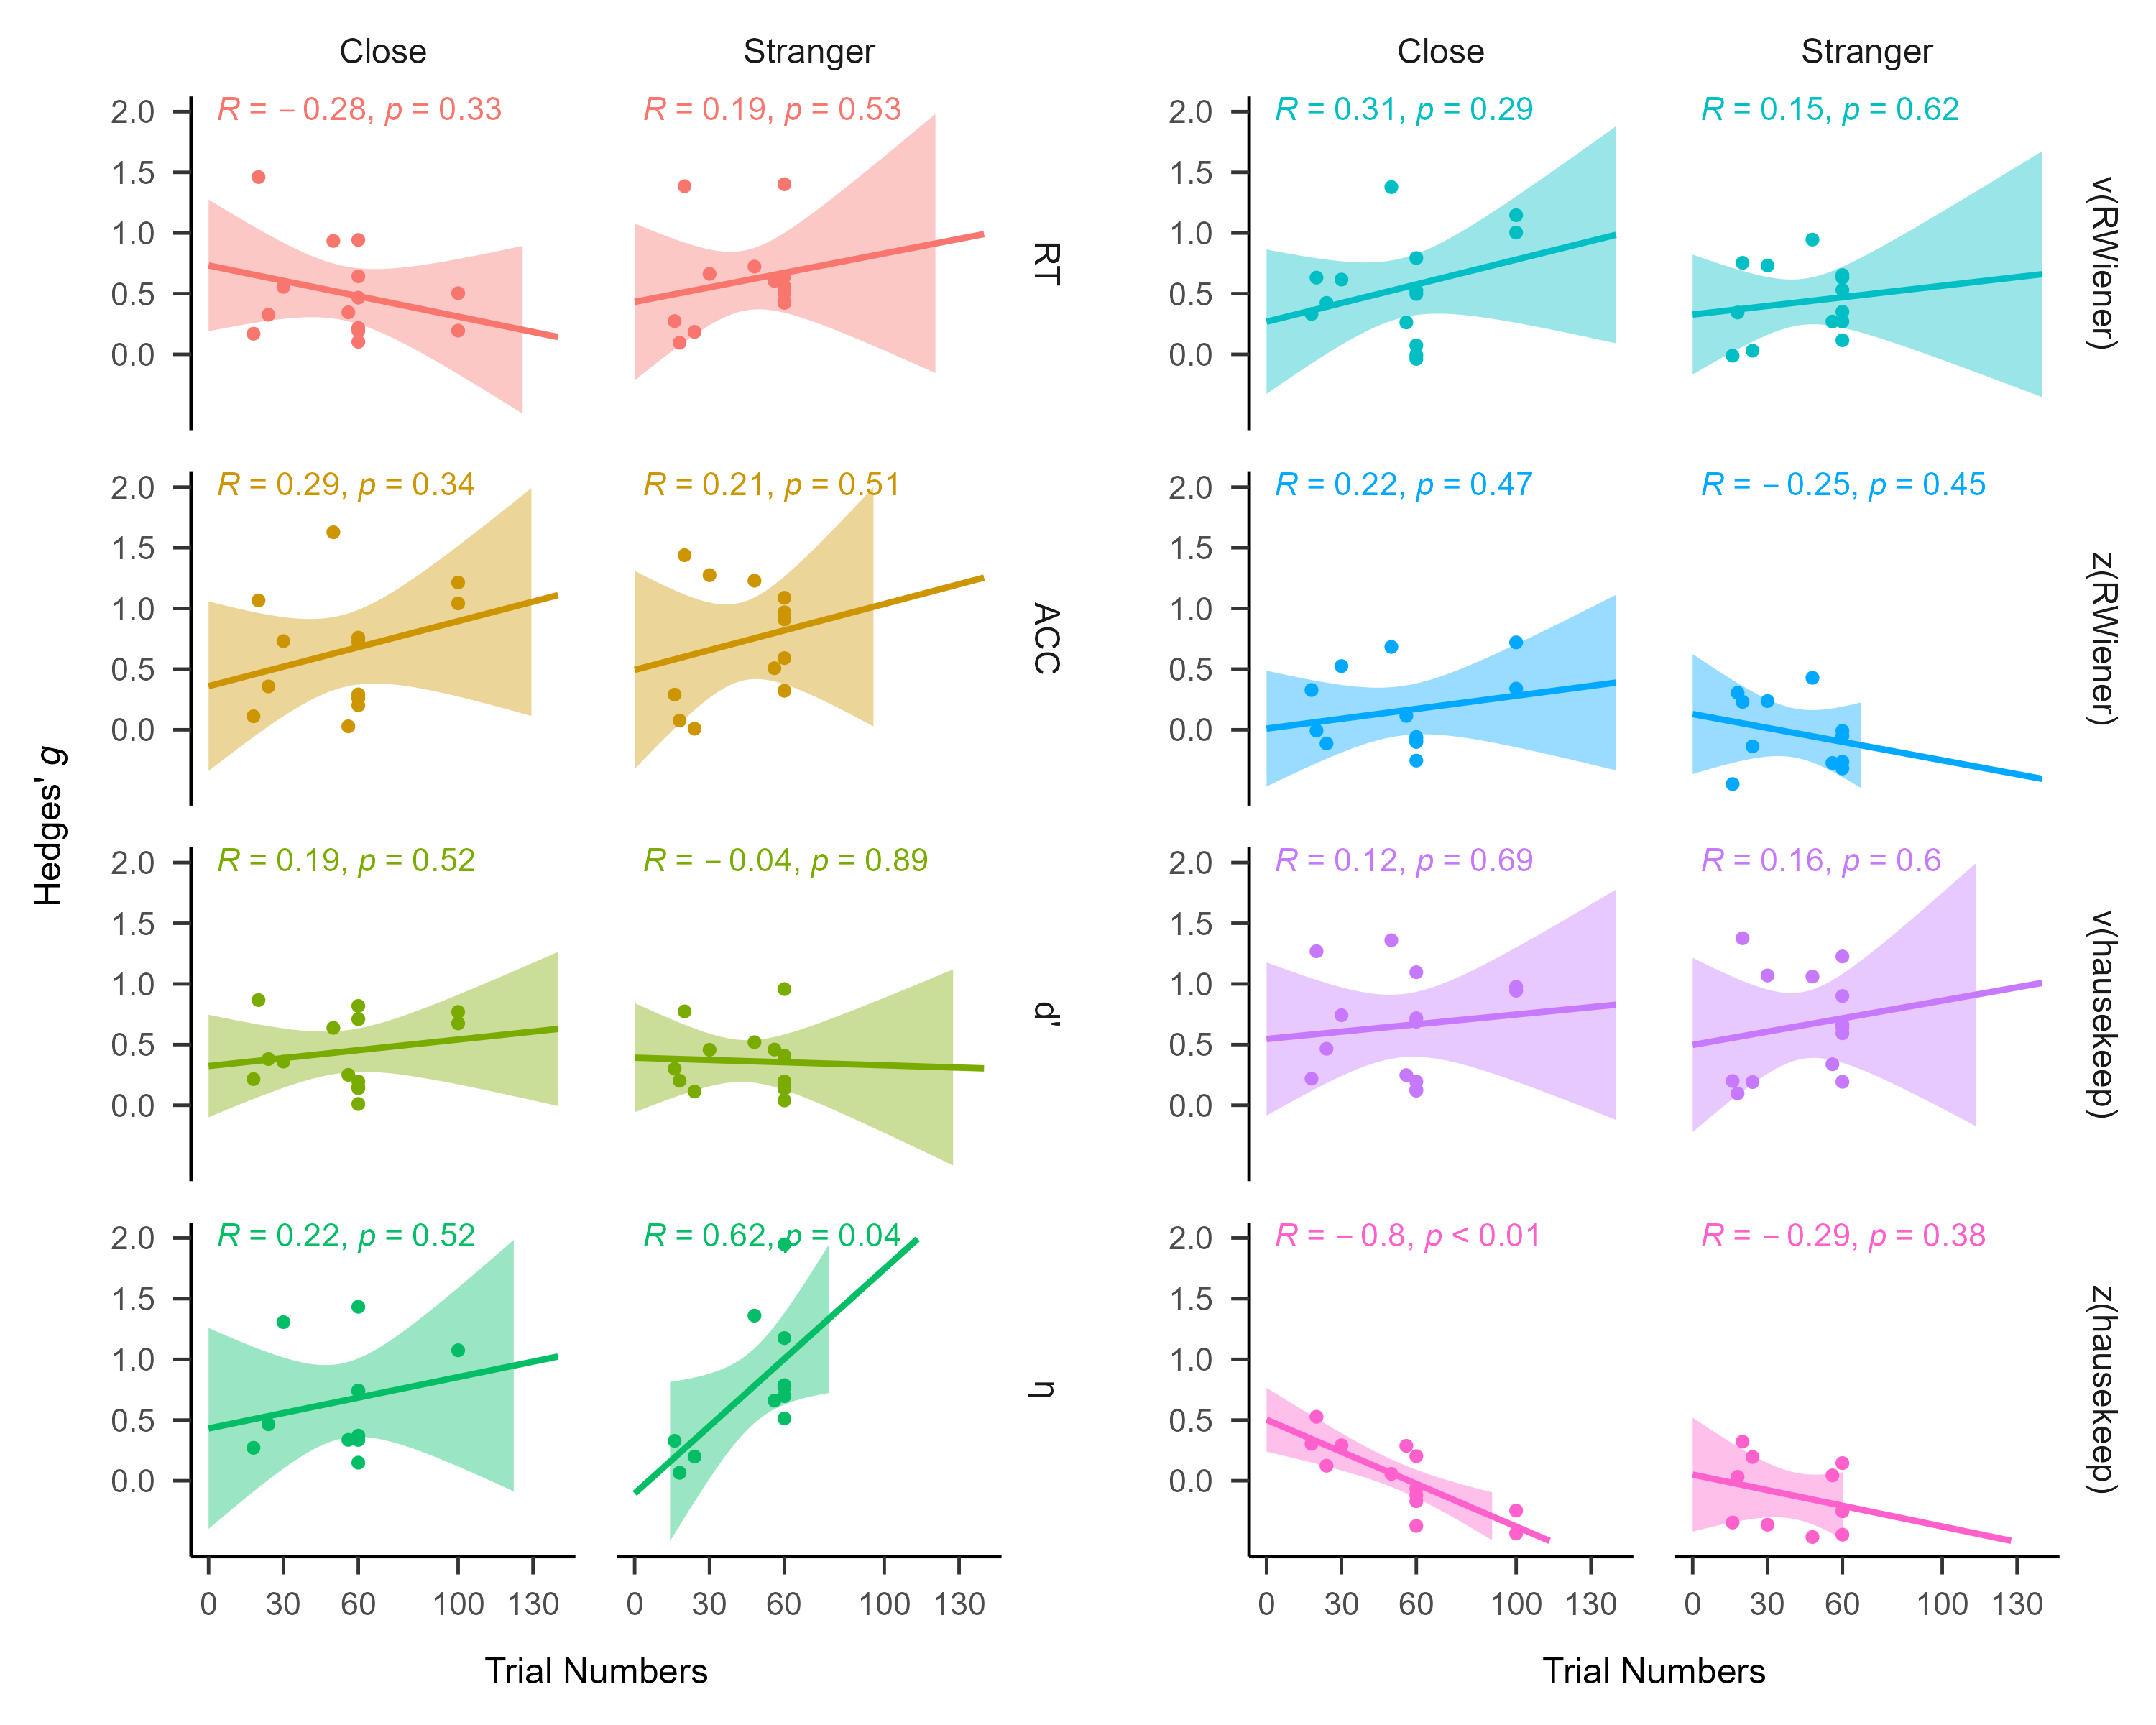
\includegraphics[width=1\textwidth]{./Figure/Fig9_cor_yi&trials.png} 
	\caption[Regression Analysis Between Trial Numbers and Effect Size (Hedges’ \textit{g}) Using Different SPE Measures]{Regression Analysis Between Trial Numbers and Effect Size (Hedges’ \textit{g}) Using Different SPE Measures.  \textit{Note}: The vertical axis represents the effect size (Hedges’ \textit{g}), and the horizontal axis represents trial numbers. Each facet represents one SPE measures.
	}\label{fig:g_nTrial}
\end{figure}

It's important to emphasize that here we only conducted simple regression analysis of these variables. This analysis was not part of the pre-registered plan, and our primary aim was not to provide a well-validated improvement for the SPMT. Nevertheless, taking into account the noteworthy correlation observed between the number of trials and Monte Carlo split-half reliability, our results indicated that when employing the SPMT paradigm for individual difference, achieving higher reliability would likely require an increase in the number of conducted trials.
\clearpage
\printbibliography
%\bibliography{sn-bibliography}% common bib file
%% if required, the content of .bbl file can be included here once bbl is generated
%%\input sn-article.bbl
\end{document}
